\documentclass[12pt,english,nohyper]{tufte-handout}\usepackage[]{graphicx}\usepackage[]{color}
%% maxwidth is the original width if it is less than linewidth
%% otherwise use linewidth (to make sure the graphics do not exceed the margin)
\makeatletter
\def\maxwidth{ %
  \ifdim\Gin@nat@width>\linewidth
    \linewidth
  \else
    \Gin@nat@width
  \fi
}
\makeatother

\definecolor{fgcolor}{rgb}{0.345, 0.345, 0.345}
\newcommand{\hlnum}[1]{\textcolor[rgb]{0.686,0.059,0.569}{#1}}%
\newcommand{\hlstr}[1]{\textcolor[rgb]{0.192,0.494,0.8}{#1}}%
\newcommand{\hlcom}[1]{\textcolor[rgb]{0.678,0.584,0.686}{\textit{#1}}}%
\newcommand{\hlopt}[1]{\textcolor[rgb]{0,0,0}{#1}}%
\newcommand{\hlstd}[1]{\textcolor[rgb]{0.345,0.345,0.345}{#1}}%
\newcommand{\hlkwa}[1]{\textcolor[rgb]{0.161,0.373,0.58}{\textbf{#1}}}%
\newcommand{\hlkwb}[1]{\textcolor[rgb]{0.69,0.353,0.396}{#1}}%
\newcommand{\hlkwc}[1]{\textcolor[rgb]{0.333,0.667,0.333}{#1}}%
\newcommand{\hlkwd}[1]{\textcolor[rgb]{0.737,0.353,0.396}{\textbf{#1}}}%

\usepackage{framed}
\makeatletter
\newenvironment{kframe}{%
 \def\at@end@of@kframe{}%
 \ifinner\ifhmode%
  \def\at@end@of@kframe{\end{minipage}}%
  \begin{minipage}{\columnwidth}%
 \fi\fi%
 \def\FrameCommand##1{\hskip\@totalleftmargin \hskip-\fboxsep
 \colorbox{shadecolor}{##1}\hskip-\fboxsep
     % There is no \\@totalrightmargin, so:
     \hskip-\linewidth \hskip-\@totalleftmargin \hskip\columnwidth}%
 \MakeFramed {\advance\hsize-\width
   \@totalleftmargin\z@ \linewidth\hsize
   \@setminipage}}%
 {\par\unskip\endMakeFramed%
 \at@end@of@kframe}
\makeatother

\definecolor{shadecolor}{rgb}{.97, .97, .97}
\definecolor{messagecolor}{rgb}{0, 0, 0}
\definecolor{warningcolor}{rgb}{1, 0, 1}
\definecolor{errorcolor}{rgb}{1, 0, 0}
\newenvironment{knitrout}{}{} % an empty environment to be redefined in TeX

\usepackage{alltt}
\usepackage[T1]{fontenc}
\usepackage[utf8]{inputenc}
\usepackage{longtable}
\usepackage{wrapfig}
\usepackage{hyperref}
\usepackage{graphicx}
\usepackage[space]{grffile}
\usepackage{geometry}
\usepackage{pgffor}
\usepackage{calc}
\usepackage{enumitem}
\usepackage{microtype}
\usepackage{tabularx}
\usepackage{floatrow}
\IfFileExists{upquote.sty}{\usepackage{upquote}}{}
\begin{document}



\begin{fullwidth}
\makeatletter\setlength\hsize{\@tufte@fullwidth}\makeatother
% latex table generated in R 3.1.3 by xtable 1.7-4 package
% Wed Jul 29 14:44:31 2015
\begin{longtable}{r|lr|r}
  \hline
mpg & cyl & disp & hp \\ 
  \hline
21.00 & 6.00 & 160.00 & 110.00 \\ 
  21.00 & 6.00 & 160.00 & 110.00 \\ 
  22.80 & 4.00 & 108.00 & 93.00 \\ 
  21.40 & 6.00 & 258.00 & 110.00 \\ 
  18.70 & 8.00 & 360.00 & 175.00 \\ 
  18.10 & 6.00 & 225.00 & 105.00 \\ 
  14.30 & 8.00 & 360.00 & 245.00 \\ 
  24.40 & 4.00 & 146.70 & 62.00 \\ 
  22.80 & 4.00 & 140.80 & 95.00 \\ 
  19.20 & 6.00 & 167.60 & 123.00 \\ 
   \hline
\hline
\caption{This is the mtcar dataset head.} 
\label{tab:mtcars}
\end{longtable}

\end{fullwidth}



\begin{fullwidth}
\makeatletter\setlength\hsize{\@tufte@fullwidth}\makeatother
\begin{figure}[!ht]
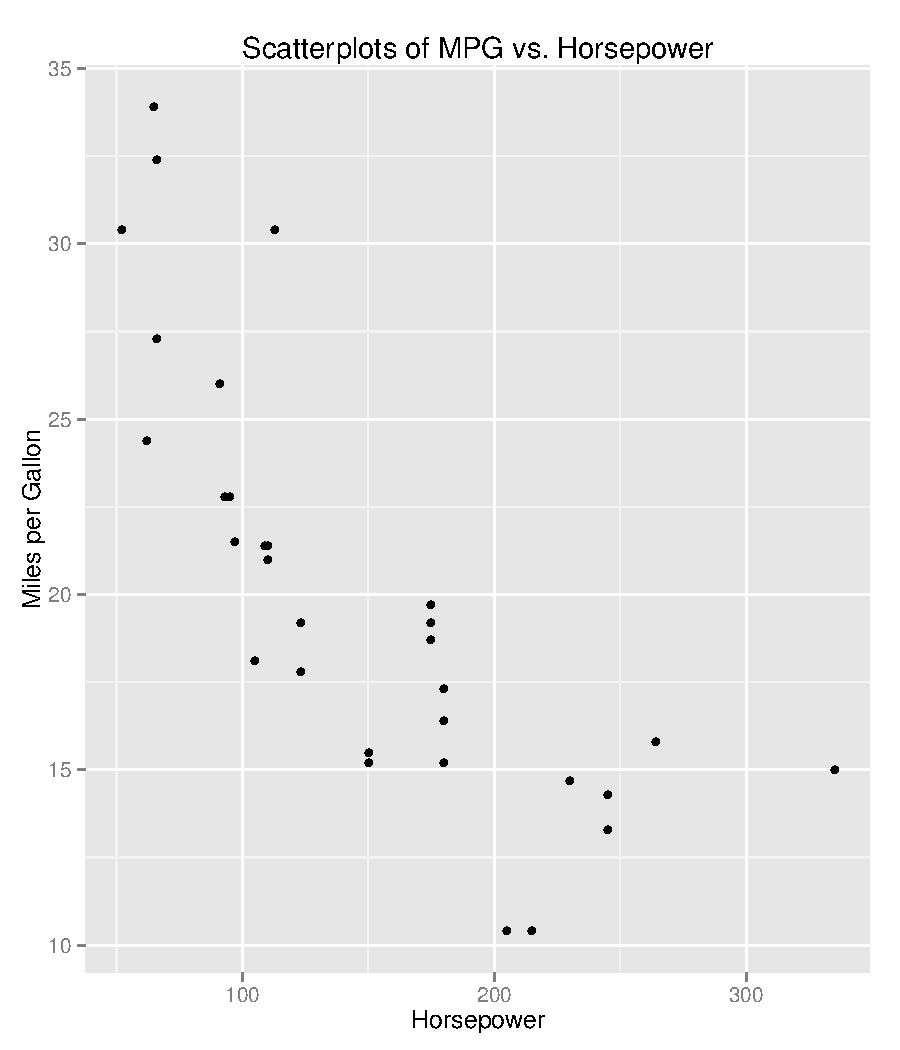
\includegraphics[width=\linewidth]{plot.pdf}
\caption{This is a plot of the mtcars dataset from R. It compares the horsepower with the miles per gallon. It uses the qplot function from ggplot2.}
\label{fig:LearningObj_summary}
\end{figure}
\end{fullwidth}

\end{document}
